\documentclass[11pt]{article}

\usepackage{latexsym}
\usepackage{amsmath}
\usepackage{amssymb}
\usepackage{amsthm}
\usepackage{graphicx}
\usepackage{wrapfig}
\usepackage{pseudocode}
\usepackage{url}
\usepackage{array}
\usepackage{amsmath}
\usepackage{algorithm}
\usepackage[noend]{algpseudocode}
\usepackage{makebox}
\usepackage{mathtools}
\usepackage{svg}
\usepackage{xcolor}
\usepackage{subfig}
\usepackage{multirow}
\usepackage{color}
\usepackage{float}
\usepackage[backref, colorlinks=true, citecolor=red, urlcolor=blue, pdfauthor={Jyh-Ming Lien}]{hyperref}


\newcommand{\handout}[5]{
  \noindent
  \begin{center}
  \framebox{
    \vbox{
      \hbox to 5.78in { {\bf } \hfill #2 }
      \vspace{4mm}
      \hbox to 5.78in { {\Large \hfill #5  \hfill} }
      \vspace{2mm}
      \hbox to 5.78in { {\em #3 \hfill #4} }
    }
  }
  \end{center}
  \vspace*{4mm}
}

\newcommand{\lecture}[4]{\handout{#1}{#2}{#3}{#4}{#1}}

\newtheorem{theorem}{Theorem}
\newtheorem{corollary}[theorem]{Corollary}
\newtheorem{lemma}[theorem]{Lemma}
\newtheorem{observation}[theorem]{Observation}
\newtheorem{proposition}[theorem]{Proposition}
\newtheorem{definition}[theorem]{Definition}
\newtheorem{claim}[theorem]{Claim}
\newtheorem{fact}[theorem]{Fact}
\newtheorem{assumption}[theorem]{Assumption}

% 1-inch margins, from fullpage.sty by H.Partl, Version 2, Dec. 15, 1988.
\topmargin 0pt
\advance \topmargin by -\headheight
\advance \topmargin by -\headsep
\textheight 8.9in
\oddsidemargin 0pt
\evensidemargin \oddsidemargin
\marginparwidth 0.5in
\textwidth 6.5in

\parindent 0in
\parskip 1.5ex
%\renewcommand{\baselinestretch}{1.25}

\begin{document}

\lecture{Midterm Exam Report}{Fall 2015}{Yunjoo Park}{Advance Algorithm Programming}

\section{Summary of the two methods}
A \textit{Voronoi diagram} of a given point set $P$ is the subdivision of the plane into $n$ cells based on distance to points, one for each site of $P$, with the property that a point $q$ lies in the cell corresponding to a site $p_i$ if and only if $dist(q, p_i ) < dist(q, p_j )$ for each $p_j \in P$ with $j \ne i$\cite{computational-geometry-book}. A \textit{Centroidal Voronoi Tessellation} (CVT) is a special type of Voronoi diagrams. In the CVT, the point of each voronoi cell is the center of mass. Especially, a \textit{Weighted Centroidal Voronoi Diagram} (WCVT) is a CVT in which each centroid is weighted according to a certain function. 
There are two methods to generate stipple drawings from images using weighted centroidal Voronoi diagrams. Both are based on the paper, "Weighted Voronoi Stipples"\cite{weighted-voronoi-stipples}. One is implemented by hedcuter. The other is implemted by voronoi method. Both generate well-spaced sets of points.
\subsection{hedcuter method}
This method is one way to generate stipple drawings from input image. This uses weighted centroidal voronoi diagram. Input is any image file and output is svg file. The program could have options below.
\begin{table}[hbt]
\centering
\begin{tabular}{|l||l|l|l|}  
\hline
Parameter & Arg. & default & Description\\
\hline\hline
-debug & X & false & Output with debugging information\\  
\hline
-n & O & 1000 & Sample size\\
\hline
-uniform\_radius & X & false & True, then all disks have the same radius\\
\hline
-radius & O & 1 &
\vtop{\hbox{\strut  If uniform\_disk is true, all disks have the disk size of the value.}\hbox{\strut Otherwise, the largest disks will have the disk size of the value.}} \\
\hline
-iteration & O & 100 & Centroidal voronoid tessellation iteration limit\\
\hline
-maxD & O & 1.01f & Max of site displacement\\
\hline
-black & X & false & True, then black disk\\
\hline
\end{tabular}
\caption{Hedcuter method's options}
\label{hedcutermethodoptions}
\end{table}

This program uses Discrete Stippling algorithm\cite{weighted-voronoi-stippling} to stipple an image quickly.

\begin{figure}[hbt]
\centering
\begin{minipage}{0.7\textwidth}

\begin{algorithm}[H]
\caption{Discrete Stippling}
\label{discretestippling}
\begin{algorithmic}
\ForAll{pixel positions $(x, y) \in [0,1]$ x $[0,1]$} 

	\State Map image value at $(x, y)$ to stipple level $l$
	\State Copy stipples on level $l$ inside $(x-\frac{1}{2}, y-\frac{1}{2})$ x $(x+\frac{1}{2}, y+\frac{1}{2})$
\EndFor
\end{algorithmic}
\end{algorithm}
\end{minipage}
\end{figure}

\clearpage
In the program, build process undergoes several steps. 
\begin{description}
  \item[First] Initialize sample points
  \item[Second] Compute a Weighted Voronoi Tessellation
	\begin{enumerate}
	  \item compute voronoi
	  \item move the site to the center of its coverage
	\end{enumerate}
  \item[Third] Create disks
\end{description}
The method use 256 as the number required in a pure black image. We call the number $N$.
\\ \\
First of all, hedcuter generates sample initial $n$ points. To be specific, $n$ is initialized by \textit{user}, or default value is 1000. For generating random points, it uses RNG (Random Number Generator). The random points are generated and distributed uniformly. The hedcuter calculates their value based on each color. If the point is close to black, the value is close to 0. On the contrary, if the point is close to white, the value is close to 1. This value is used to determines which points are appropriate. The points are decided whether to keep or not by comparing the value with a random number sampled from the gaussian distribution. Thus, the black has higher probability.
\\ \\
Second part is main of the hedcuter. At first, the hedcuter copies all points to \textit{site of cells} and calculate \textit{distance} for cells. The distance of each cell is obtained by converting its color intensity to distance value [0, 1] by equation (\ref{eq:colortodist}). Let $indensity(c)$ be the color intensity and $distance(c)$ be the distance of the stipple.

\begin{equation}
distance(c) = \frac{\left(N-intensity\left(c\right)\right)*1.0f}{N}
\label{eq:colortodist}
\end{equation}

And then, sort cells using heap. The next step is about propagation. For each cell, the hedcuter calculate new distance of its neighbors. Neighbors are the points which are 3X3 matrix around the stipple.

\begin{equation}
distance_{new}(neighbor) = distance(c) + distance(neighbor)
\label{eq:distance}
\end{equation}

If the calculated distance is less than the distance of the neighbor, push the neighbor to heap with the new distance. Finally, after the propagation step, the hedcuter collects cells by pushing points to ceverage of corresponding cell and removes empty cells. For the collected cells, the hedcuter computes weighted average distance of each cell and updates the site of the cell to the new position using the distance. Repeat these process while satisfying the following conditions.
\begin{itemize}
  \item the max of the displacement of site at each iteration  $<$ max\_site\_displacement (1.01f)
  \item the number of iterations $<$ iteration\_limit (option: -iteration)
\end{itemize}

\subsection{voronoi method}
This method is also one way to generate stipple drawings from input image. This uses weighted centroidal voronoi diagram. Input file must be a PNG image. The program could have options below. Specifically, input and output are required\cite{saliences}.
\begin{table}[hbt]
\centering
\begin{tabular}{|l||l|l|l|}  
\hline
Param. & Arg. & default & Description\\
\hline\hline
-I & O &  & Must be a PNG file.\\  
\hline
-O & O &  & The name of the file to output\\
\hline
-s & O & 4000 & The number of stipple points to render.\\
\hline
-c & X & OFF & Off, output in black and white\\
\hline
-t & O & 0.1 & The cut-off point for the convergence of the stippled output.\\
\hline
-n & X & OFF & Stipple points will not overlap.\\
\hline
-f & X & OFF & ON, then all stipple points have the equal size of radius.\\
\hline
-z & O & 1.0 & The radius of each stipple is multiplied by this value.\\
\hline
-p & O & 5 & Controls the tile size of centroid computations.\\
\hline
-l & X & OFF & ON, then produce an output log.\\
\hline
\end{tabular}
\caption{Voronoi method's options}
\label{voronoimethodoptions}
\end{table}
\\
As I mentioned before, in CVT, each generating point lies exactly on the centroid of its voronoi region. The centroid of a region is defined as 
\begin{equation}
C_i = \frac{\int_{A} x\rho(x), dA}{\int_{A} \rho(x), dA}
\label{eq:centroid}
\end{equation}
where $A$ is the region of the cell, $x$ is the position and $\rho(x)$ is the density function. A centroidal voronoi diagram is a minimum-energy configuration in the sense that it minimize $\int_{A}\rho(x){|C_i-x|}^2$.\cite{weighted-voronoi-stipples}
This program uses Lloyd's algorithm\cite{weighted-voronoi-stippling} to generate a centroidal Voronoi diagram from any set of generating points.
\begin{figure}[hbt]
\centering
\begin{minipage}{0.7\textwidth}

\begin{algorithm}[H]
\caption{Lloyd's method}
\label{lloydmethod}
\begin{algorithmic}
\While{generating points $x_i$} 
	\State Compute the Voronoi diagram of $x_i$
	\State Compute the centroids $C_i$ using equation (\ref{eq:centroid})
	\State Move each generating point $x_i$ to its centroid $C_i$
\EndWhile
\end{algorithmic}
\end{algorithm}
\end{minipage}
\end{figure}
\\
The algorithm find evenly spaced sets of points in subsets of Euclidean spaces, and partitions of these subsets into well-shaped and uniformly sized convex cells. That is, Under the algorithm, a voronoi diagram become a centroidal voronoi diagram through relaxation step.
\clearpage
The program consists of the following several steps.
\begin{description}
  \item[First] Create stippler
  \item[Second] Loop while (average displacement $>$ threshold)
	\begin{enumerate}
	  \item distribute stipples
		\begin{enumerate}
	     \item create voronoi diagram	
	     \item redistribute stipples
		\end{enumerate}
	\end{enumerate}
  \item[Third] Render
\end{description}

In the first step, creates initial stipples. The second step is the main part. Firstly, in the \textit{createVoronoiDiagram()} part, generates a voronoi diagram using stipples. Second, in the \textit{redistributeStipples()} part, calcuates the centroid of a cell using edges of the cell. To be specific, in the process of calcuating the centroid, creates and computes clip lines. Each clip line is extension of each edge. Thus, the clip lines form a polygon. Tests whether each point around the stipple is outside of the polygon or not. gets the density from image for inside points, calculates the density of the cell, and returns the center and radius of the cell. Updates stipples of voronoi diagram with the centroid. After updating, calculates the average displacement of stipples, denoted by $t$. Repeat this second step while $t$ is greater than the \textit{threshold}.

\section{Comparison of the two methods}
\subsection{Do you get the same results by running the same program on the same image multiple times?}%2.1
\begin{enumerate}
	\item Hedcuter
	\begin{figure}[htbp]
	  \centering
	  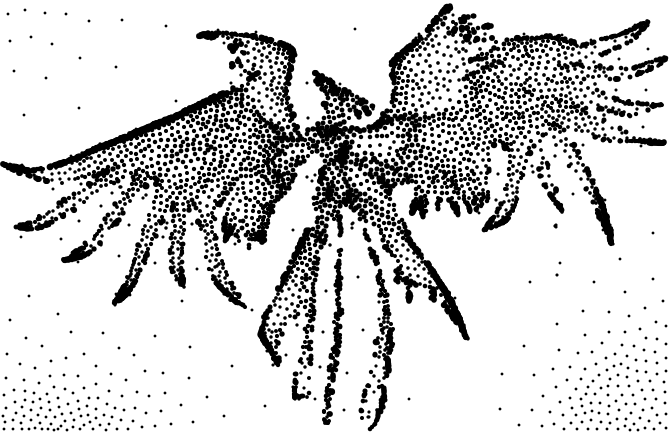
\includegraphics[width=.23\textwidth]{FIGS/hedcut/svg/phoenix-5000-h1}
	  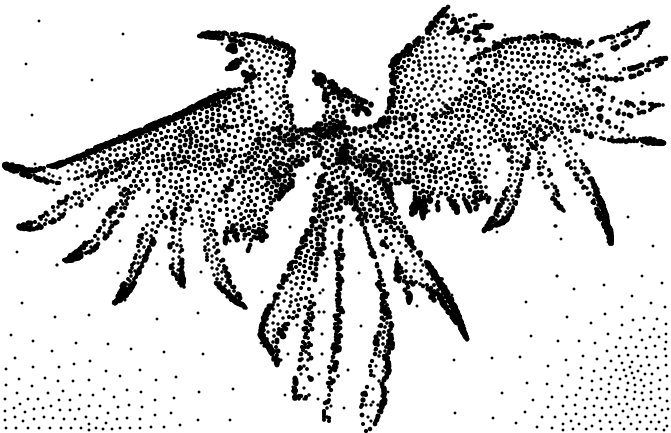
\includegraphics[width=.23\textwidth]{FIGS/hedcut/svg/phoenix-5000-h2}
	  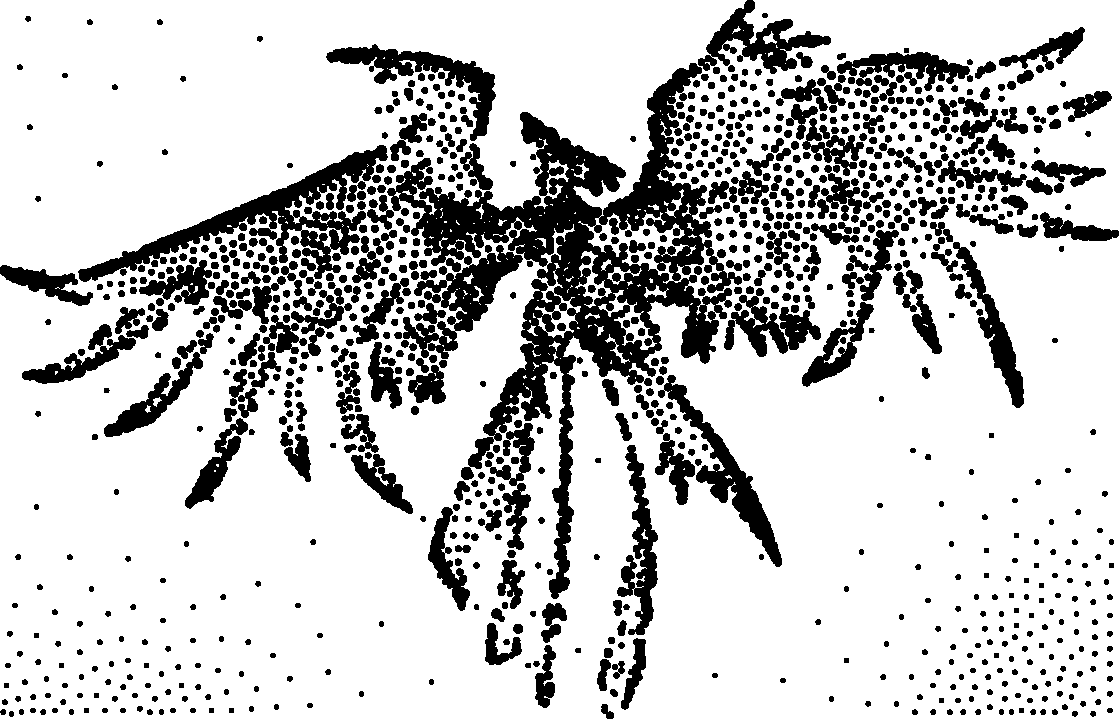
\includegraphics[width=.23\textwidth]{FIGS/hedcut/svg/phoenix-5000-h3}
	  \caption{phoenix with 5000}
	  \label{fig:hedcuterphoenix}
	\end{figure}

	\item Voronoi
	\begin{figure}[htbp]
 	 \centering
 	 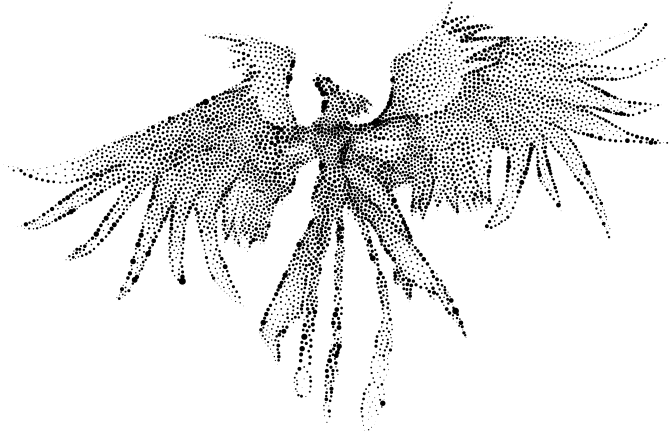
\includegraphics[width=.23\textwidth]{FIGS/voronoi/svg/phoenix-5000-v1}
 	 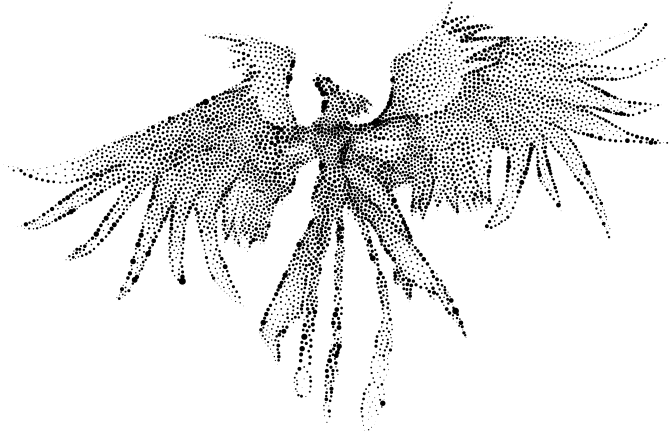
\includegraphics[width=.23\textwidth]{FIGS/voronoi/svg/phoenix-5000-v2}
 	 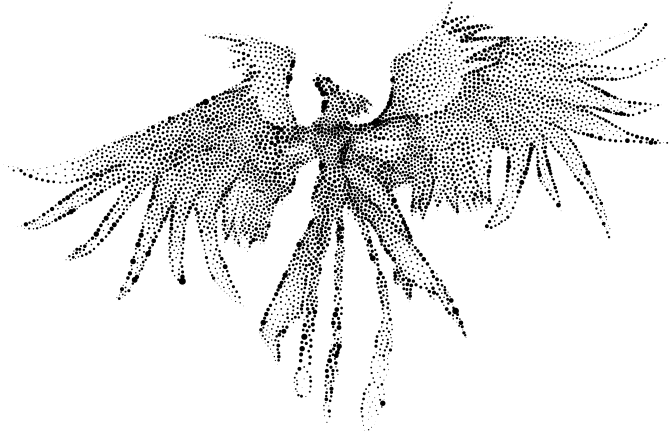
\includegraphics[width=.23\textwidth]{FIGS/voronoi/svg/phoenix-5000-v3}
 	 \caption{phoenix with 5000}
	\end{figure}
\end{enumerate}
While I got the different outputs by running the hedcuter program on the same image multiple times, I obtained the same outputs by running the voronoi program. The hedcuter generates initial points randomly and make a CVT under limit iteration and given max site displacement. Since initial points set are different, the results of propagation are also changed. On the other hand, the voronoi program has the same initial points and repeats the series of process until the average of displacement of points is small enough. Thus, I could get the same output multiple times.

\subsection{If you vary the number of the disks in the output images, do these implementations produce the same distribution in the final image? If not, why?}%2.2
Figure \ref{fig:varydiskhedcut} and \ref{fig:varydiskvoronoi} show the output image of klaymen of Hedcuter and Voronoi. outputBoth methods produce the different distribution in the final image when the the number of the disks in the output images varies. As the number of the disks increases, they generate the more detailed results.

	\begin{figure}[ht] 
	\begin{center} 
	\subfloat[2981 disks]{
		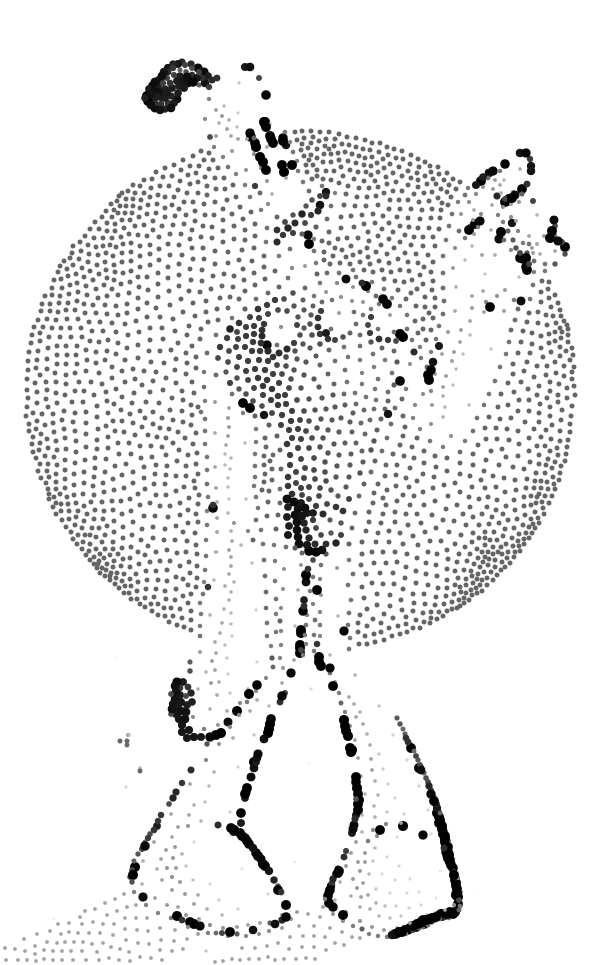
\includegraphics[width=0.18\textwidth]{FIGS/hedcut/svg/klaymen-3000-h}}
		\hspace{5mm}
	\subfloat[4943 disks]{
		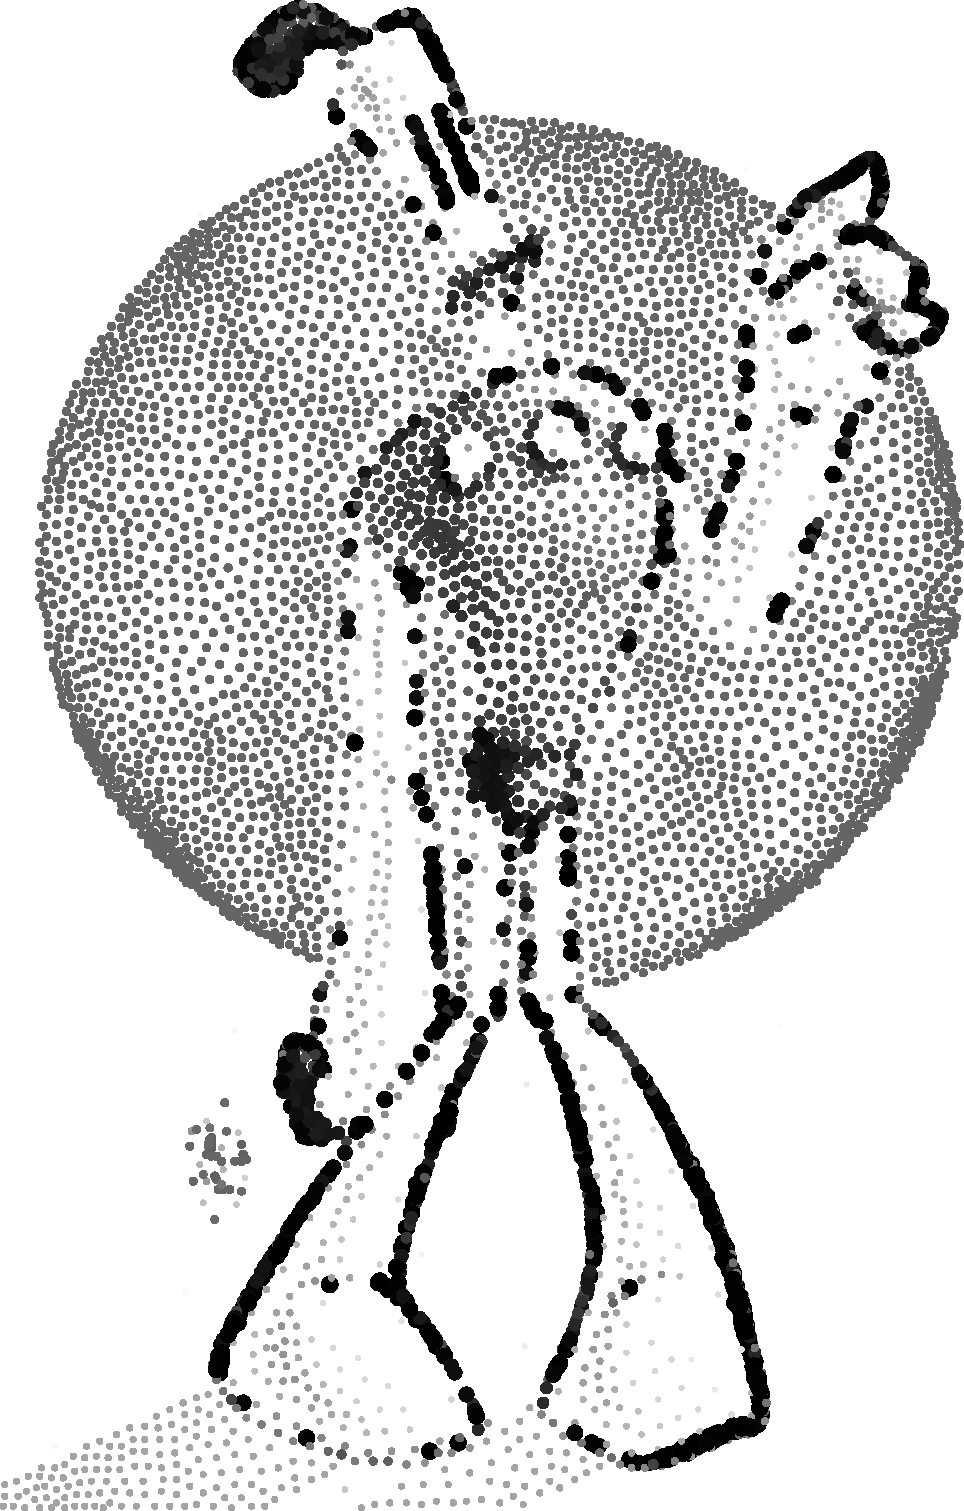
\includegraphics[width=0.18\textwidth]{FIGS/hedcut/svg/klaymen-5000-h}}
	\hspace{5mm}
	\subfloat[9829 disks]{
		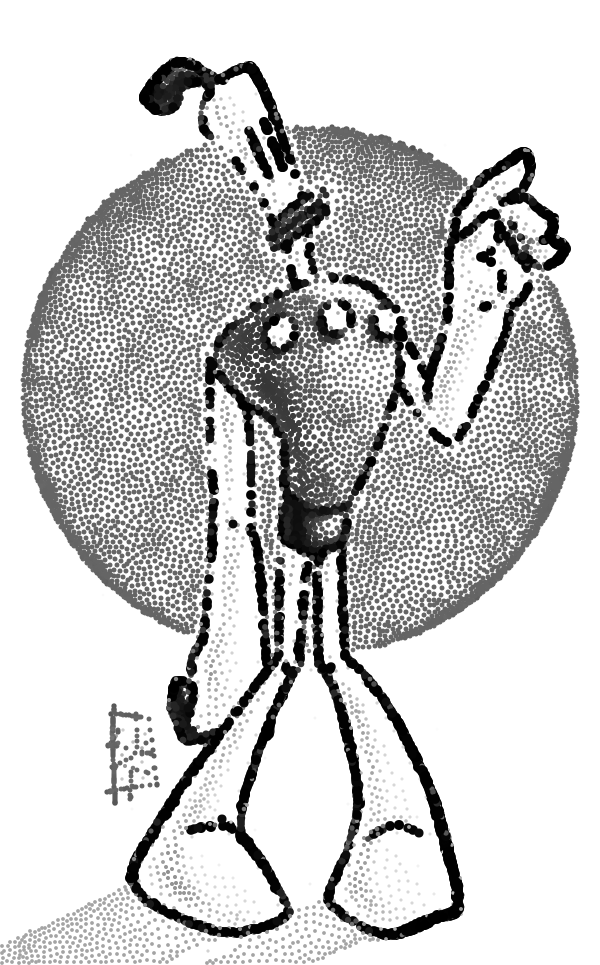
\includegraphics[width=0.18\textwidth]{FIGS/hedcut/svg/klaymen-10000-h}}
	\hspace{5mm}
	\subfloat[55070 disks nonblack]{
		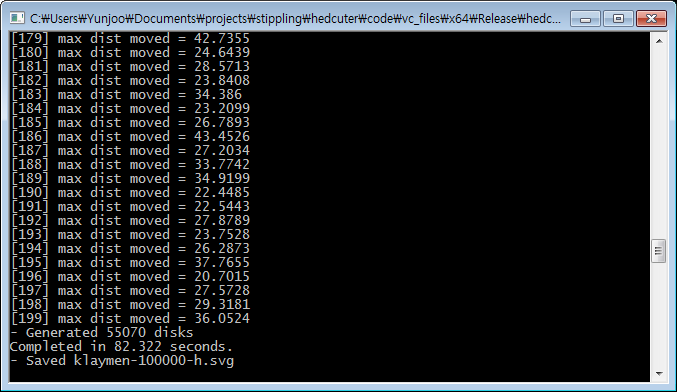
\includegraphics[width=0.18\textwidth]{FIGS/hedcut/svg/klaymen-100000-h-nonblack}}
	\caption{Hedcuter klaymen}
	\label{fig:varydiskhedcut} 
	\end{center} 
	\end{figure}
	\begin{figure}[ht] 
	\begin{center} 
	\subfloat[1000 stipples]{
		\includegraphics[width=0.18\textwidth]{FIGS/voronoi/svg/klaymen-1000-v}}
		\hspace{5mm}
	\subfloat[5000 stipples]{
		\includegraphics[width=0.18\textwidth]{FIGS/voronoi/svg/klaymen-5000-v}}
		\hspace{5mm}
	\subfloat[20000 stipples]{
		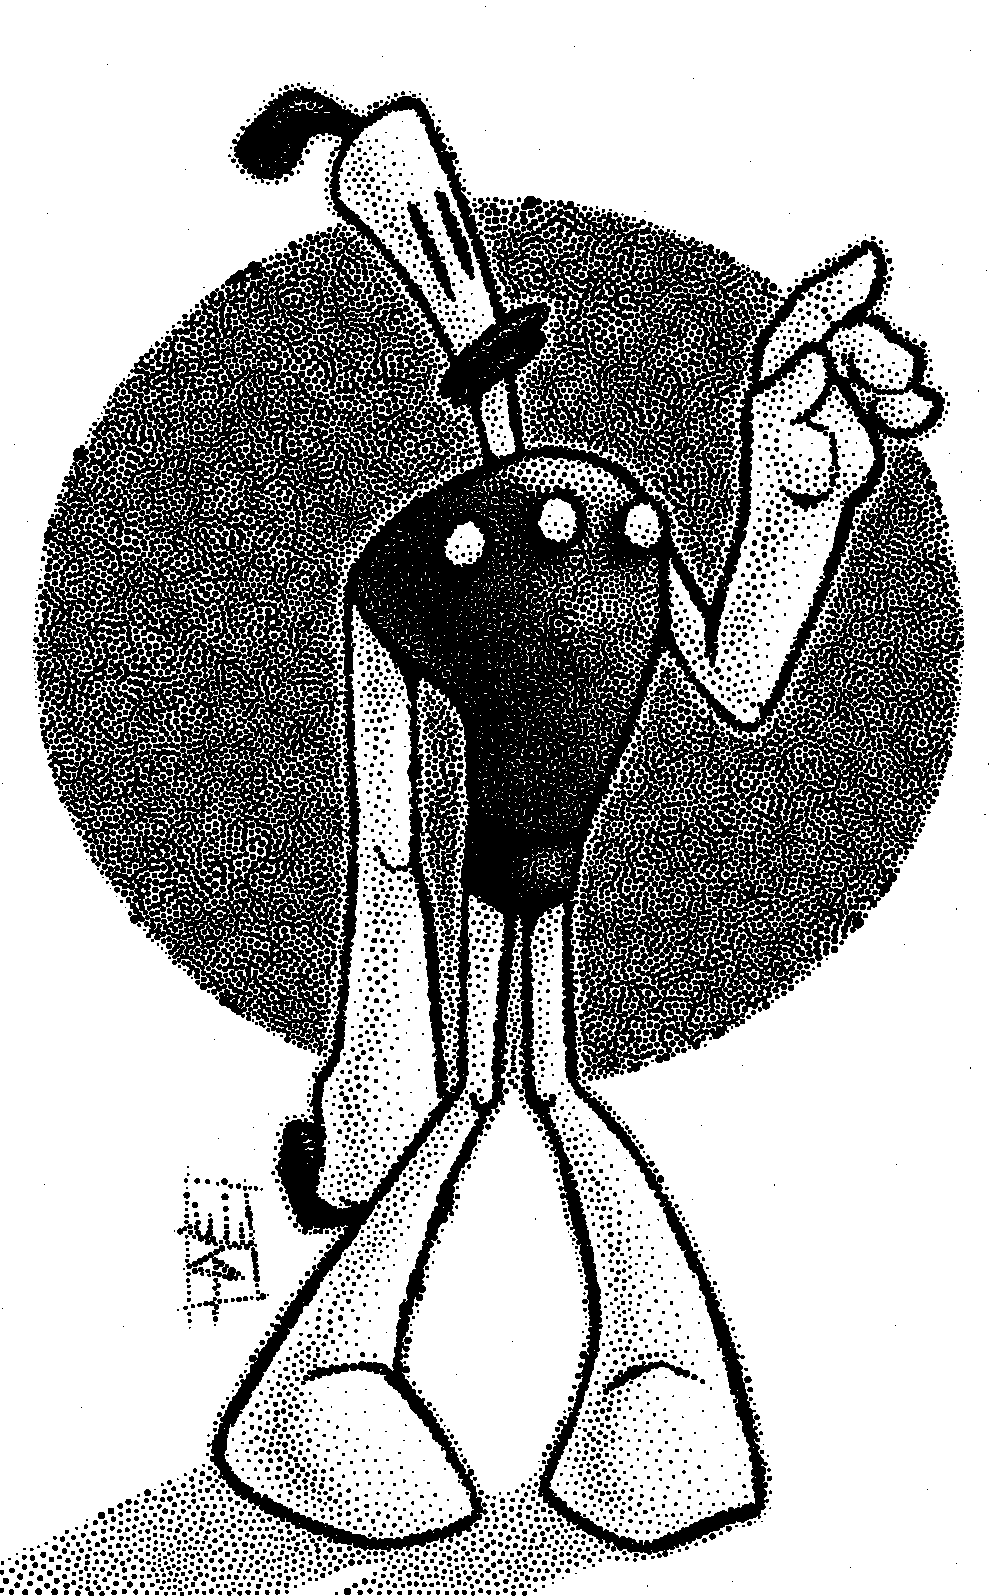
\includegraphics[width=0.18\textwidth]{FIGS/voronoi/svg/klaymen-20000-v}}
		\hspace{5mm}
	\subfloat[100000 stipples]{
		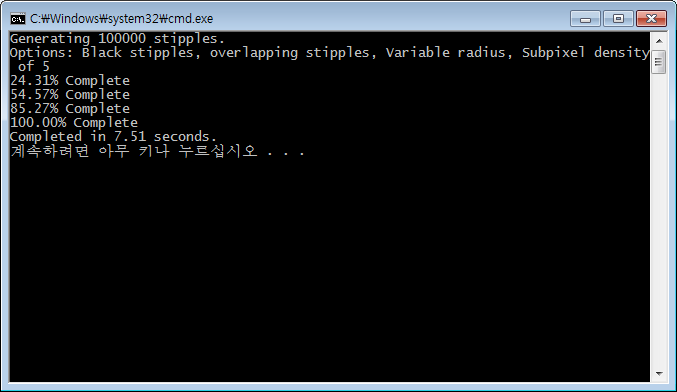
\includegraphics[width=0.18\textwidth]{FIGS/voronoi/svg/klaymen-100000-v}}
	\caption{Voronoi klaymen} 
	\label{fig:varydiskvoronoi}
	\end{center} 
	\end{figure}
\clearpage

\subsection{If you vary the number of the disks in the output images, is a method faster than the other?}%2.3
I could not assure that one method is faster than the other. In the hedcuter method, there are some points which oscillate after a few iteration in some cases. Thus, if there is no iteration limit, it will take infinite time because some points will oscillate infinitely. In the voronoi method, the more I increase the number of points, it takes the small number of iteration. Figure \ref{fig:klaymenrunningtimevoronoi} and \ref{fig:einsteinrunningtimevoronoi} show elapsed time of the voronoi as the number of stipples is varied. As the number of points increases, the method becomes faster. However, the elapsed time increases again when the number of points goes beyond a certain level. This is because it takes too much time for each iteration even though there are few iteration.

\begin{figure}[hbpt] 
	\begin{center} 
	\subfloat[1000 stipples]{
		\includegraphics[width=0.4\textwidth]{FIGS/voronoi/running_time/klaymen-1000-v}}
		\hspace{5mm}
	\subfloat[5000 stipples]{
		\includegraphics[width=0.4\textwidth]{FIGS/voronoi/running_time/klaymen-5000-v}}

	\subfloat[20000 stipples]{
		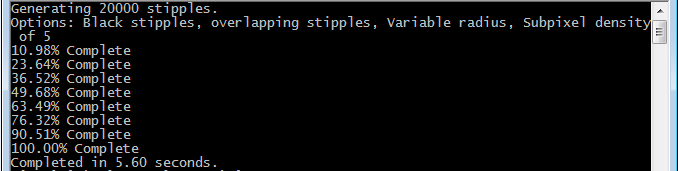
\includegraphics[width=0.4\textwidth]{FIGS/voronoi/running_time/klaymen-20000-v2}}
		\hspace{5mm}
	\subfloat[100000 stipples]{
		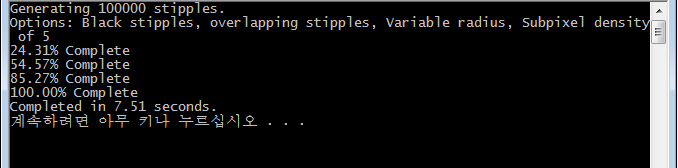
\includegraphics[width=0.4\textwidth]{FIGS/voronoi/running_time/klaymen-100000-v2}}
	\caption{Elapsed time of Klaymen of Voronoi as a function of the number of stipples} 
	\label{fig:klaymenrunningtimevoronoi}
	\end{center} 
\end{figure}

\begin{figure}[hbpt] 
	\begin{center} 
	\subfloat[100 stipples]{
		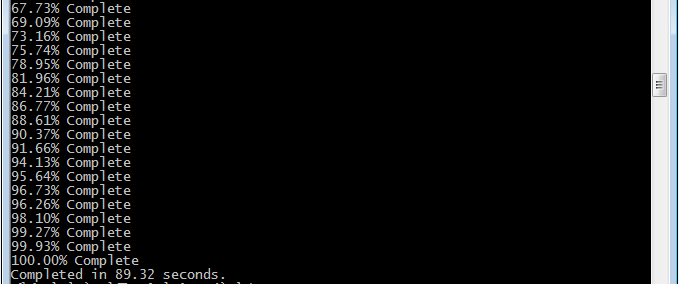
\includegraphics[width=0.4\textwidth]{FIGS/voronoi/running_time/einstein-100-v2}}
		\hspace{5mm}
	\subfloat[5000 stipples]{
		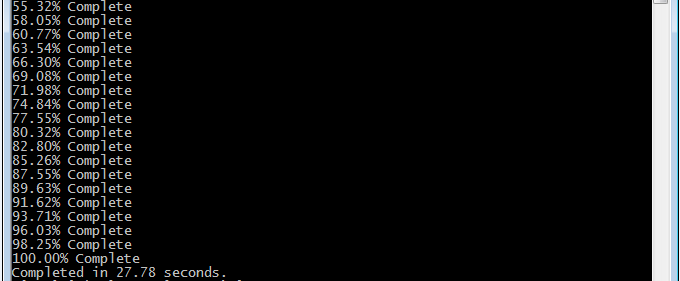
\includegraphics[width=0.4\textwidth]{FIGS/voronoi/running_time/einstein-5000-v2}}

	\subfloat[250000 stipples]{
		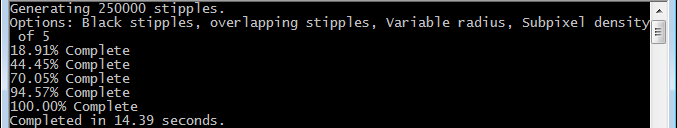
\includegraphics[width=0.4\textwidth]{FIGS/voronoi/running_time/einstein-250000-v2}}
		\hspace{5mm}
	\subfloat[10000000 stipples]{
		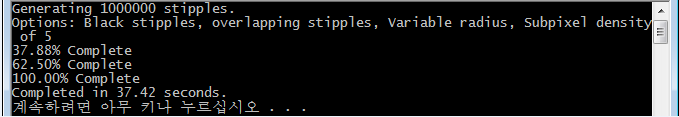
\includegraphics[width=0.4\textwidth]{FIGS/voronoi/running_time/einstein-10000000-v2}}
	\caption{Elapsed time of Klaymen of Voronoi as a function of the number of stipples} 
	\label{fig:einsteinrunningtimevoronoi}
	\end{center} 
\end{figure}


\subsection{Does the size (number of pixels), image brightness or contrast of image increase or decrease their difference?}

\subsection{Does the type of image (human vs. machine, natural vs. urban landscapes, photo vs.painting, etc) increase or decrease their difference?}
\subsection{Are the outputs of these stippling methods different the hedcut images created by artists (e.g. those from the Wall Street Journal)?}

\section{Improvement of hedcuter method}

\bibliographystyle{plain}
\bibliography{report}

\end{document}


